We will now study the most simple hyperbolic surface the once punctured torus.
A usual torus can not have a hyperbolic structure, it has naturally a flat structure as the quotient $\mathbb{R}^2 / \mathbb{Z}^2$.
But his changes when one study the one punctured torus. It is a torus $S$ where we choose a point $p$ and remove it (or just marked it).


The construction of this object can be done in two manier at least.
For the first construction, we give a fundamental domaine in the upper half plane. It is a hexagone with two vertex "at infinity" on the real line. We glue each arc to the symetric one.



\begin{figure}[h]
\centering
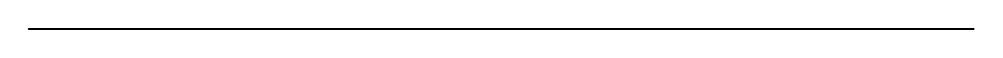
\begin{tikzpicture}[scale=1,cap=round]
\tkzInit[xmin=-4, xmax=4, ymin=0, ymax=3]
\tkzClip
%Draw circle
\tkzDefPoint(0,0){O} %define origin
\tkzDefPoint(-2,0){x1}
\tkzDefPoint(2,0){x2}
\tkzDefPoint(-3,0){y1}
\tkzDefPoint(3,0){y2}
\tkzDefPoint(-2.25,0){c1}
\tkzDefPoint(2.25,0){c2}

\tkzDrawCircle[thick, fill=gray!30](O,y1){circleOy}
\tkzDrawCircle[thick, fill=white](O,x1){circleOx}

\tkzDrawCircle[thick, fill=white](x1,c1){circlex1}
\tkzDrawCircle[thick, fill=white](x2,c2){circlex2}
\tkzDrawCircle[thick, fill=white](y1,c1){circley1}
\tkzDrawCircle[thick, fill=white](y2,c2){circley2}

\draw[thick] (-6, 0) -- (6, 0); %horizontal line

\end{tikzpicture}
\caption{A fundamental domain of a punctured torus}
\end{figure}


A second construction is given by the representation of the fushian group. Given two hyperbolic isomorphism of $\mathbb{H}$ $A$ and $B$ with different fixed point on $\delta \mathbb{H}$. We ask in addition that the commutator $H := ABA^{-1}B^{-1}$ should be a parabolic element.

\subsection{First properties}

The geometry of the one punctured torus make it simple to discuss closed curves and laminations.
\begin{rmq}
Given two generators $\alpha$ and $\beta$ of $\pi_1(S)$, two closed curves non homotopically trivial which intersect one, one can parametrize all other lamination.
Indeed a given lamination $\lambda \in \mathcal{ML}$ is determined by the couple $(i(\alpha,\lambda),i(\beta,\lambda))$ where $i(.,.)$ is the geometric intersection number.
\end{rmq}

The collaring is a powerful tool in this situation since two closed curves can not be disjoint. The length of one is bound below by the collar of the other. So we have the following lemma:

\begin{lem}
If $X$ is a hyperbolic surface homeomorph to the once punctured torus with a simple closed curve of lenght inferior at $ln(3+2 \sqrt{2})$, then there is only one simple closed curve representing the systole.
\end{lem}

Moreover, we have this useful lemma to estimate the length of the systole function in the Teichmuller space.

\begin{lem}
Pick $\gamma$ a simple closed geodesic, and $X \in \mathcal{T}(S_{1,1)}$, if $X$ has Fenchel-Nielsen coordinate $(L,\frac{p}{q})$ with respect to $\gamma$, where $gcd(p,q)=1$ and $\frac{p}{q} \in ]0;1[$, then \[
C_1(L) e^{\frac{-L}{2q}} < l_{sys}(X) < C_2(L) e^{\frac{-L}{2q}}
\]
where $C_1(L)$, $C_2(L)$ both limits to $4$ when $p$, $q$ are fixed and $L$ goes to $\infty$
\end{lem}

\begin{proof}
Let $R(L)$ be the length of the shortest geodesic arc with endpoints on $\gamma$. We have \[
R(L)= 2 log(coth(L/4))=2 log(\frac{e^{l/2}+1}{e^{l/2}-1})
\]
By the collar lemma \ref{ColLem}.
Then if we take $\alpha$ a simple closed curve that intersect $\gamma$, $q$ times exactly, we obtain the following inequality with $a=l_\alpha(X)$ \[
q R(a) < L < q R(a) + \frac{qa}{2}
\]
Reorganizing the termes we have \[
e^{-a/4}tanh(a/4) < e^{-L/2q} < tanh(a/4)
\]
As $a \rightarrow 0$ then $L \rightarrow \infty$
\[
C_1(L) e^{\frac{-L}{2q}} < a < C_2(L) e^{\frac{-L}{2q}}
\]
To complete the proof , we need to show that the length of $\alpha$ is shorter than any other geodesic closed curves, but with the collar lemma there is only one systole whose length goes to $0$ and this is the case for $\alpha$ as $L \rightarrow \infty$.
%TODO detailler la preuve

%If we don't do any approximation we have \[
%2 ln(\frac{1+e^{-L/2q}}{1-e^{-L/2q}}) < a
%\]
\end{proof}

\subsection{Rate of mixing of the Earthquake flow}

If $\rho$ is a positive real number we will note $J(\rho)= \{t \in \mathbb{R} , l_\gamma(t) \leq \rho \}$, where $l_{\lambda,\gamma}(t)=l_{\gamma}(E_t(X,\lambda))$.

To shorten the notation we will use $\mu=i(\lambda_p,\gamma)$ and $\epsilon_\gamma = min_{t \in \mathbb{R}} l_\gamma (t)$.


Kerckoff show in \cite{NielsenRealizationPr} the following proprities of the earthquake flow.

\begin{prop}
For every $(x,\lambda) \in \mathcal{PT}^1$ and every $\gamma \in \Gamma^S$, the function $l_{\lambda,\gamma}: t \mapsto l_\gamma(E_t(x,\lambda))$ is $C^1$ and convex.

If $i(\gamma,\lambda)=0$ then l_{\lambda,\gamma} is constant, and if $i(\gamma,\lambda)>0$ then $l_{\lambda,\gamma}$ is proper, with derivative strictly increasing and given by \begin{equation}
\frac{d}{dt}l_{\lambda,\gamma}(t)= \int_{\gamma_t}cos(\theta_{y,t})d \lambda(y)
\end{equation}
Here $\gamma_t$ is the geodesic representative of $\gamma$ in $E_t(X,\lambda)$, and $\theta_{\gamma,t}$ is the angle of the intersection between $\lambda$ and $\gamma_t$.
\end{prop}

With this proposition we can easily show that \[
$-i(\lambda_p,\gamma) < \frac{d}{dt}l_{p,\gamma}(t) < i(\lambda_p,\gamma)$
\]

The following lemma can be found in \cite{articleMetW}.

\begin{lem}\label{LemFra}

There are constants $\rho$ and $C$, depending only on $S$, such that for any $(X, \lambda) \in \mathcal{PT}^1$,$\gamma \in \Gamma^S$
and all $t\in J(\rho)$, \[
\mu |t-t_\gamma |-C \epsilon_\gamma \leq l_{\lambda,\gamma}(t) \leq \mu |t- t_\gamma | + \epsilon_\gamma
\]

\end{lem}

We now fix a $\epsilon$, such has $2 \epsilon(2+C) < min( \rho , ln(3+2 \sqrt{2}))$ and a $\mu$. Let \[
C_{\epsilon,\mu}=\{ (X,\lambda) \in \mathcal{T}(S) \times \mathcal{ML},l_{sys}(X) \in  [\frac{\epsilon}{2};\epsilon], i(\lambda,\gamma) \in [-\mu,\mu]  \}
\]
where $\gamma$ is the closed curve representing the systole. Moreover, let $D$ be the set $\{ (X,\lambda) \in \mathcal{T}(S) \times \mathcal{ML},l_{sys}(X) > ln(3+2 \sqrt{2}) \} $.

So let $X$ be a hyperbolic surface in $C_{\epsilon,\mu}$. The systole of this surface is $\gamma$ and has length $\tilde{\epsilon}$
When we earthquake $X$ along $\lambda$, the length function will reach a minimum value $\epsilon_\gamma$ at the time $t_\gamma$. Using the inequalities of lemma \ref{LemFra}, we find that \[
\frac{\tilde{\epsilon}-\epsilon_\gamma}{\mu} \leq |t_\gamma | \leq \frac{\tilde{\epsilon} + C \epsilon_\gamma}{\mu}
\]
and as $0 < \epsilon_\gamma \leq \tilde{\epsilon}$ we have $|t_\gamma| \in [0; \frac{\tilde{\epsilon}}{\mu}(1+C)]$. Injecting this in the right-hand side of inequality of lemma \ref{LemFra}, we get: \[
l_\gamma (E_t (X,\lambda)) \leq \tilde{\epsilon} (2+C) +\mu |t|
\]

Hence, for all $|t| \leq \frac{\epsilon}{\mu}(2+C) = t_{lim}$ we have that $l_\gamma(E_t(X,\lambda)) \leq 2 \epsilon (2+C)$.

Let $f_{\epsilon,\mu}$ a Lipschitz positive function with support include in $C_{\epsilon,\mu}$, $\int f_{\epsilon,\mu} > Vol(C_{\epsilon,\mu})/2$.

We take also $g$ a positive Lipschitz function with support in $D$, $K_1= \int g$ and $\| g \|_{Lip}= K_2$.
So we have:\[
|\int f_{\epsilon,\mu} \circ E_{t_{lim}} g - \int f_{\epsilon,\mu} \int g |=K_1 \int f_{\epsilon,\mu}
\]

If we have exponential mixing, we would have two constants $\tau'$ and $K_3$ such that \[
\frac{Vol(C_{\epsilon,\mu})}{2}K_1 \leq K_1 \int f_{\epsilon,\mu}
< K_2 K_3 \| f_{\epsilon,\mu} \|_{Lip} e^{-\epsilon \frac{2+C}{\mu \tau'}}
\]

Or more simply \begin{equation}
Vol(C_{\epsilon,\mu}) < K' \| f_{\epsilon,\mu} \|_{Lip} e^{-\frac{\epsilon}{\mu \tau}}
\label{equ}
\end{equation}


We can also make the hypothesis that the earthquake flow has a polynomial decay rate. We change the inequality \ref{equ} in
\begin{equation}
Vol(C_{\epsilon,\mu}) < K' \| f_{\epsilon,\mu} \|_{Lip} (\frac{\epsilon}{\mu})^{-\gamma}
\label{poly}
\end{equation}
Where $\gamma \in \mathbb{R^{+*}}$.

We should now understand the volume of $C_{\epsilon,\mu}$ and the Lipschitz norm of $f_{\epsilon,\mu}$. Note that we are interested in an upper bound of the norm and a lower bound of the volume.


One can choose $f_{\epsilon,\mu}$ to be a piecewise product of linear as follow:\[
f_{\epsilon,\mu}=g_{\epsilon}h_{\epsilon}j_{\epsilon,\mu}
\]
With
$$
g_{\epsilon} = \left \{
\begin{array}{lll}
0 & \text{if} & l_{sys} \notin [\epsilon/2;\epsilon]\\
1 & \text{if} & l_{sys} \in [\frac{4 \epsilon}{6};\frac{5 \epsilon}{6}]\\
\frac{6}{\epsilon}(l_{sys}(X)-\frac{\epsilon}{2}) & \text{if} & l_{sys} \in [\frac{\epsilon}{2};\frac{4 \epsilon}{6}]\\
\frac{-6}{\epsilon}(l_{sys}(X)-\epsilon) & \text{if} & l_{sys} \in [\frac{5 \epsilon}{6};\epsilon]
\end{array}
\right .
$$

$$
h_{\lambda} = \left \{
\begin{array}{lll}
0 & \text{if} & l_{\lambda}(X) > 1\\
1 & \text{if} & l_{\lambda}(X) \leq \frac{1}{2}\\
-2(l_\lambda(X -1)) & \text{if} & l_{\lambda}(X) \in [\frac{1}{2};1]
\end{array}
\right .
$$

$$
j_{\epsilon,\mu} = \left \{
\begin{array}{lll}
0 & \text{if} & i(\lambda,\gamma) > \mu\\
1 & \text{if} & i(\lambda,\gamma) \leq \mu/2\\
\frac{-2 }{\mu}(i(\lambda,\gamma)-\mu) & \text{if} & i(\lambda,\gamma) \in [\mu/2; \mu]
\end{array}
\right .
$$

Then we need to calculate the different Lipschitz norms of this function.

To estimate the volume of $C_{\epsilon,\mu}$, and following \cite{fu2015cusp}, we use the fact that the measure $\nu$ restricted to the space of unit-length measured laminations is equal to the Thurston volume of the unit ball.

When we will have the two previous estimation, we would know if the earthquake flow has exponential mixing rate or polynomial rate and a bound of the degree of the polynome in the last case.
